\chapter{Introduction to diagnostic medical imaging}\label{chap:imaging}

\section{Introduction}
In this chapter, we provide an overview of diagnostic medical imaging and its
history. Medical imaging is a field in medicine concerned with creating visual
representations of a body for the purpose of clinical analysis. Although medical
imaging is sometimes used for non-diagnostic purposes, we will only concern
ourselves with diagnostic medical imaging. This subbranch has the goal to
facilitate diagnosis of medical conditions without the need for invasive
procedures. Over the past fifty years, this discipline has matured
significantly, it has become indispensable in the modern age medical setting
\cite{review}.

The most important aspect of diagnostic medical imaging is image production, but
various other aspects are involved. Image processing, image display, image
recording, image transmission and image storage are all related. Modern day
Picture Archiving and Communication Systems (PACS) provide all these features.
Once the image has been captured and processed, it can be presented to a
radiologist for diagnosis. In recent years, scientists have focused on
augmenting the physician's diagnostic ability with various Computer Aided
Diagnosis (CAD) schemes. For example, algorithms based on machine learning are
able to autonomously detect lung nodules with ever increasing accuracy
\cite{ginneken}. Although some systems aim to make physicians redundant in the
long term, most experts agree that software should augment them rather than
replace them entirely.

In the next sections, we will discuss the history technical background and
recent advancements of the most important imaging modalities.

\section{Radiography}
Radiographs are the simplest form of medical imaging based on X-rays. These rays
can travel through solid objects, but attenuate based on the materials they meet
along their path. For example, when passing through a human hand, the
attenuation is stronger when passing through bones rather than through soft
tissue. The image can be recorded (in negative) on ordinary photographic paper
and processed in darkrooms. \autoref{fig:xrayhand} shows am example.

\begin{figure}[ht]
\begin{center}
  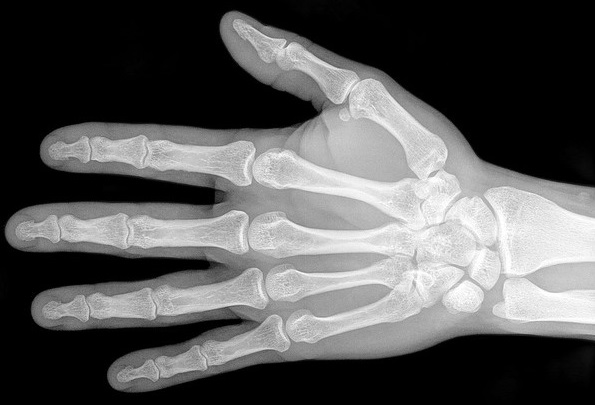
\includegraphics[width=\linewidth]{img/xrayhand.jpg}
  \caption{X-ray image of a human hand. In this negative image, bones are
  lighter because fewer X-rays managed to get through them.}
  \label{fig:xrayhand}
\end{center}
\end{figure}

\subsection{History}
Radiography builds on the work of Wilhelm Konrad R\"ontgen, a German physicist
who produced and detected X-rays for the first time on the 8 of November 1895.
These X-rays (X for unknown) had the remarkable property of being attenuated at
different rates when passing through various materials. For example, bone
strongly attenuates the X-rays while soft tissue does much less so. R\"ontgen
also discovered that the radiation can be captured on a photographic plate, just
like regular light. He presented his findings in his paper ``On a new kind or
rays'' \cite{rontgen}. This discovery earned him the Nobel Prize in Physics in
1901.

Only two weeks after his discovery he produced the first X-ray photo of his
wife's hand, after which she reportedly exclaimed: ``I have seen my death!''.
Just a couple of months later, X-rays were already being used in a clinical
setting on patients.

Note that during this time, not much was known about ionizing radiation or
radioactivity. Only a year after the discovery of X-rays did Henri Becquerel
discover radioactivity. Well known scientists such as Ernest Rutherford and
Pierre \& Marie Curie performed several more years worth of research before
realizing the true danger of prolonged exposure to this type of radiation.

\subsection{Technical background}
To better understand the internal workings of imaging devices, we present a
simplified mathematical and physical background based on the book of prof.
Suetens\cite{suetens}. X-rays are simply a form of electromagnetic waves
consisting of photons with a wavelength $\lambda$ on the order of Angstr\o ms
($10^{-10}$m). The corresponding frequency $f$ places these rays firmly in the
ionizing part of the spectrum - that is, they can cause cancer.
\autoref{fig:spectrum} shows a schematic overview of the whole spectrum. The
energy of such a wave can be calculated with the following formula, where $c$
is the speed of light and $h$ is Planck's constant.

\begin{figure}[ht]
\begin{center}
  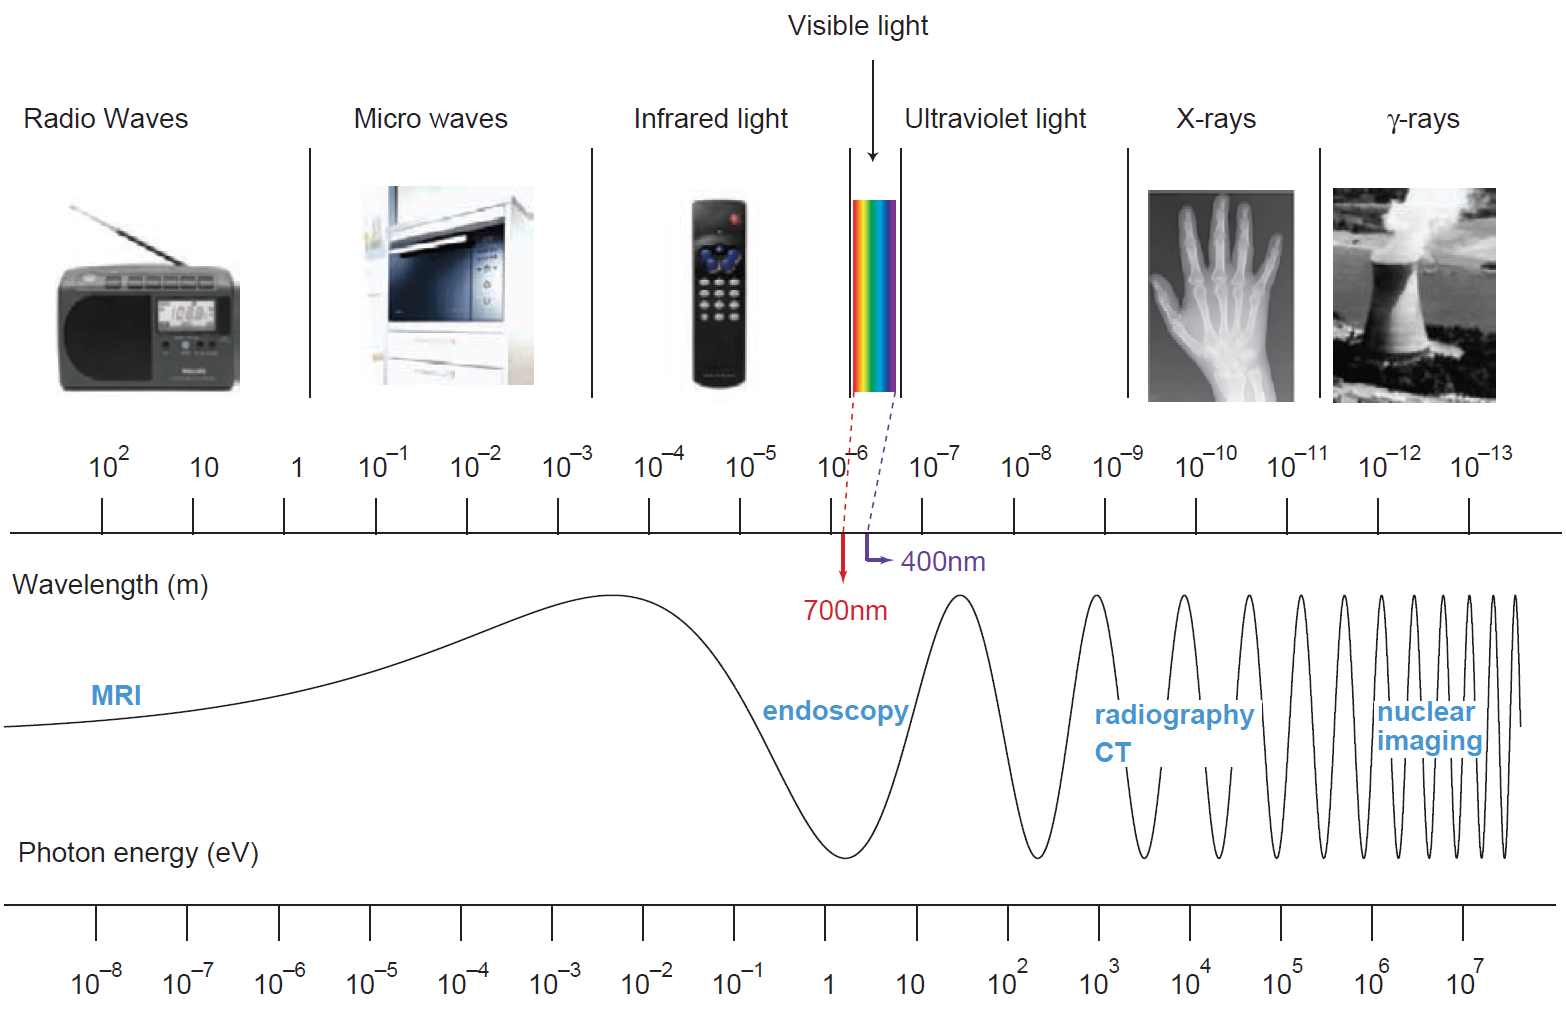
\includegraphics[width=\linewidth]{img/spectrum.png}
  \caption{The electromagnetic spectrum. \cite{suetens}}
  \label{fig:spectrum}
\end{center}
\end{figure}

\begin{equation}
	E = hf = \frac{hc}{\lambda}.
\end{equation}

This formula can of course easily be extended to include heterogeneous materials
and variable attenuation coefficients.

X-rays are generated in an X-ray tube, a vacuum tube consisting of a cathode and
an anode. Current flowing through the cathode releases electrons,
which are accelerated toward the anode by an applied voltage. Once the electrons
hit the anode, they release part of their energy in the form of X-ray photons.
Thus, the two most important settings of an X-ray scan are the applied
current multiplied by the exposure time (mA $\cdot$ s) and the applied voltage
(keV).

The attenuation of X-rays through materials can easily be modeled using an
attenuation coefficient $\mu$. The beam intensity when passed through a
homogeneous material of depth $d$ is given by: 

\begin{equation}
	I_{out} = I_{in} e^{-\mu d}.
\end{equation}

To capture X-rays, a detector is needed. Traditionally, a screen-film detector
was used. The familiar photographic film alone is very inefficient
at capturing X-rays: only about 2\% of all photons are absorped. Because X-rays
are ionizing, the applied dose cannot simply be increased to improve the
image quality. Instead, an intensifier screen is used in front of the film. This
screen contains heavy chemical elements, whose electrons are excited by the
incoming photons. When returning to their original state, these electrons emit
visible light that can better be captured by the film, raising the absorption
efficiency to about 50\%.

Besides ordinary radiography, special classes such as fluoroscopy and
mammography exist. Fluoroscopy generates time-lapse recordings instead of still
images. With modern technology, tens of frames per second are achievable. Of
course, each frame must be shot at a very low exposure rate to minimize patient
risk. Mammography on the other hand produces images of the human breast. The
challenge here is to generate very high resolution images, so that small masses
can be seen.

\subsection{Recent advancements}\label{ssec:recentradio}
Relatively recently, X-ray systems have moved away from analogue detectors
towards digital ones. Much like digital photographs, digital X-ray scans are far
easier to store, copy, post-process and share. On top of that, they typically
have a much wider exposure range making them more tolerant to over- and
underexposure. These detector systems use storage phosphors to temporarily hold
the absorbed radiation instead of immediately releasing it in the form of
photons. This phenomenon is caused by electron traps in the doped material.
Later, this phosphor can be read out pixel-wise using an optical detector array
and a laser that gives the electrons enough energy to escape their trap. The
main obstacle for this paradigm shift was the large pixel size. Pixels of 1 mm make
it much more difficult for a radiologist to analyze the image in its digital
form. Only by the time pixels could be as small as 0.1 mm did the medical world
embrace digital detectors \cite{review}.

Even newer devices use active matrix flat panel detectors. These detectors are
able to produce near real time images where storage phosphors and older
technologies required minutes or more of processing time.

\subsubsection{A note on image quality}\label{sssec:imgquality}
The quality of an image can be expressed in three dimensions: resolution,
contrast and noise \cite{suetens}.

Resolution is sometimes simply stated as the pixel density (dots per inch).
However, this only provides an upper bound because in practise neighbouring
pixels can be correlated. For example, due to the imperfect nature of the
recording equipment, a single point can appear as blurred blob on the resulting
image. This blob is called the Point Spread Function (PSF), and is a better
measure for the actual image resolution. If the resolution is isotropic, the
Line Spread Function (LSF) - measured in distinguishable line pairs per mm
(lp/mm) - can also be used. Alternatively, the Optical Transfer Function (OTF,
sometimes also MTF) representing amplitude and phase shifts of a sinusoidal
target can be used. In fact, this OTF is nothing more than the Fourier transform
of the PSF or LSF.

Second, contrast is the intensity difference between neighbouring regions of the
image. More formally, contrast at a given frequency is the amplitude component
of the image at that frequency in the frequency domain (calculated using the
Fourier transform). Contrast is dependent on the whole imaging process, but also
on the size and shape of the objects in the image. 

Third, noise is partly the result of interfering phenomena. Yet, it is also
inherent to the electromagnetic radiation itself because the waves themselves
are stochastic processes. An important measure is the Signal to Noise Ratio
(SNR) or, more appropriately, the Contrast to Noise Ratio (CNR). Noise can be
estimated by examining the result of an scan with no object present, a so-called
flat-field image. Another measure for the amount of noise is the Wiener
spectrum.

Another frequently used metric called the Detective Quantum Efficiency (DQE) can
compare various technologies without being dependent on the object being imaged.

\begin{equation}
DQE(f) = \frac{SNR(f)_{out}^2}{SNR(f)_{in}^2}
\end{equation}

In addition to these elements, sometimes artifacts appear on scans. The
causes of these artificial image features vary widely depending on the image
modality used and can also be caused by excessive post-processing.

\subsection{Future expectations}
Ever since CT scanners - and to a lesser extent MRI scanners - made their way
into hospitals, they have taken over many of the tasks traditionally reserved
for basic radiography. This declining trend is expected to continue in the
foreseeable future.

\section{X-ray computed tomography}
One step up from basic radiography is computed tomography (Greek for ``slice
writing''). The goal here is to create image slices of patients in the
cross-sectional plane rather than the frontal plane. To accomplish this, the X-ray
source-detector pair is rotated around the patient. From this raw data, a
so-called filtered back projection algorithm can reconstruct the whole cross
section image. A computer is needed to make sense of the output, hence the
\emph{computed} in the name. \autoref{fig:ctscan} shows an example of a chest
CT scan and \autoref{fig:ctscanner} shows an actual scanner.

\begin{figure}[ht]
\begin{center}
  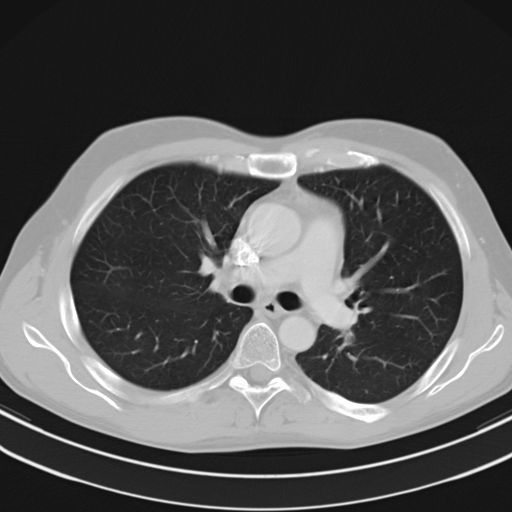
\includegraphics[width=0.4\linewidth]{img/ct-thorax.jpg}
  \caption{Example of a thoracic CT scan. The heart is clearly visible in the
  center. Bones (ribs, sternum, spine) are also easy to spot in the periphery.
  The large black area represents the lungs filled with air.}
  \label{fig:ctscan}
\end{center}
\end{figure}

\subsection{History}
Before computed tomography became possible, some simpler techniques were already
being used to obtain slices from inside the patient's body. These techniques
were called (non-computed) tomography. One example is linear tomography,
where source and detector move on parallel tracks, but in opposite directions,
during the scanning process. This way, one section of the patient is always
projected on the same spot of the detector, while the rest is averaged out.
Obviously, these techniques where nowhere near as accurate as the CT scanners we
know today.

In 1917, Johann Radon - an Austrian mathematician - presented the first
algorithm to reconstruct a function from its projections: the Radon transform
\cite{radon}.

After World War II, the development of computers gained momentum, but it would
still take a long while before the ``computed" in ``computed tomography" became
feasible. In the 1960's, the South African Allan McLeod Cormack continued
working on the mathematics invented by Radon \cite{ctreview}. A decade later, in
1972, the first operational brain CT scanner (the EMI scanner) was designed by
Godfrey Hounsfield, an Englishman. A scan took about 5 minutes, after which a
computer performed calculation for up to 150 minutes. The final output was a
80px $\times$ 80px image. Cormack and Hounsfield shared the 1979 Nobel Prize in
Physiology or Medicine for their work related to CT scans \cite{ctbook}.

\begin{figure}[ht]
\begin{center}
  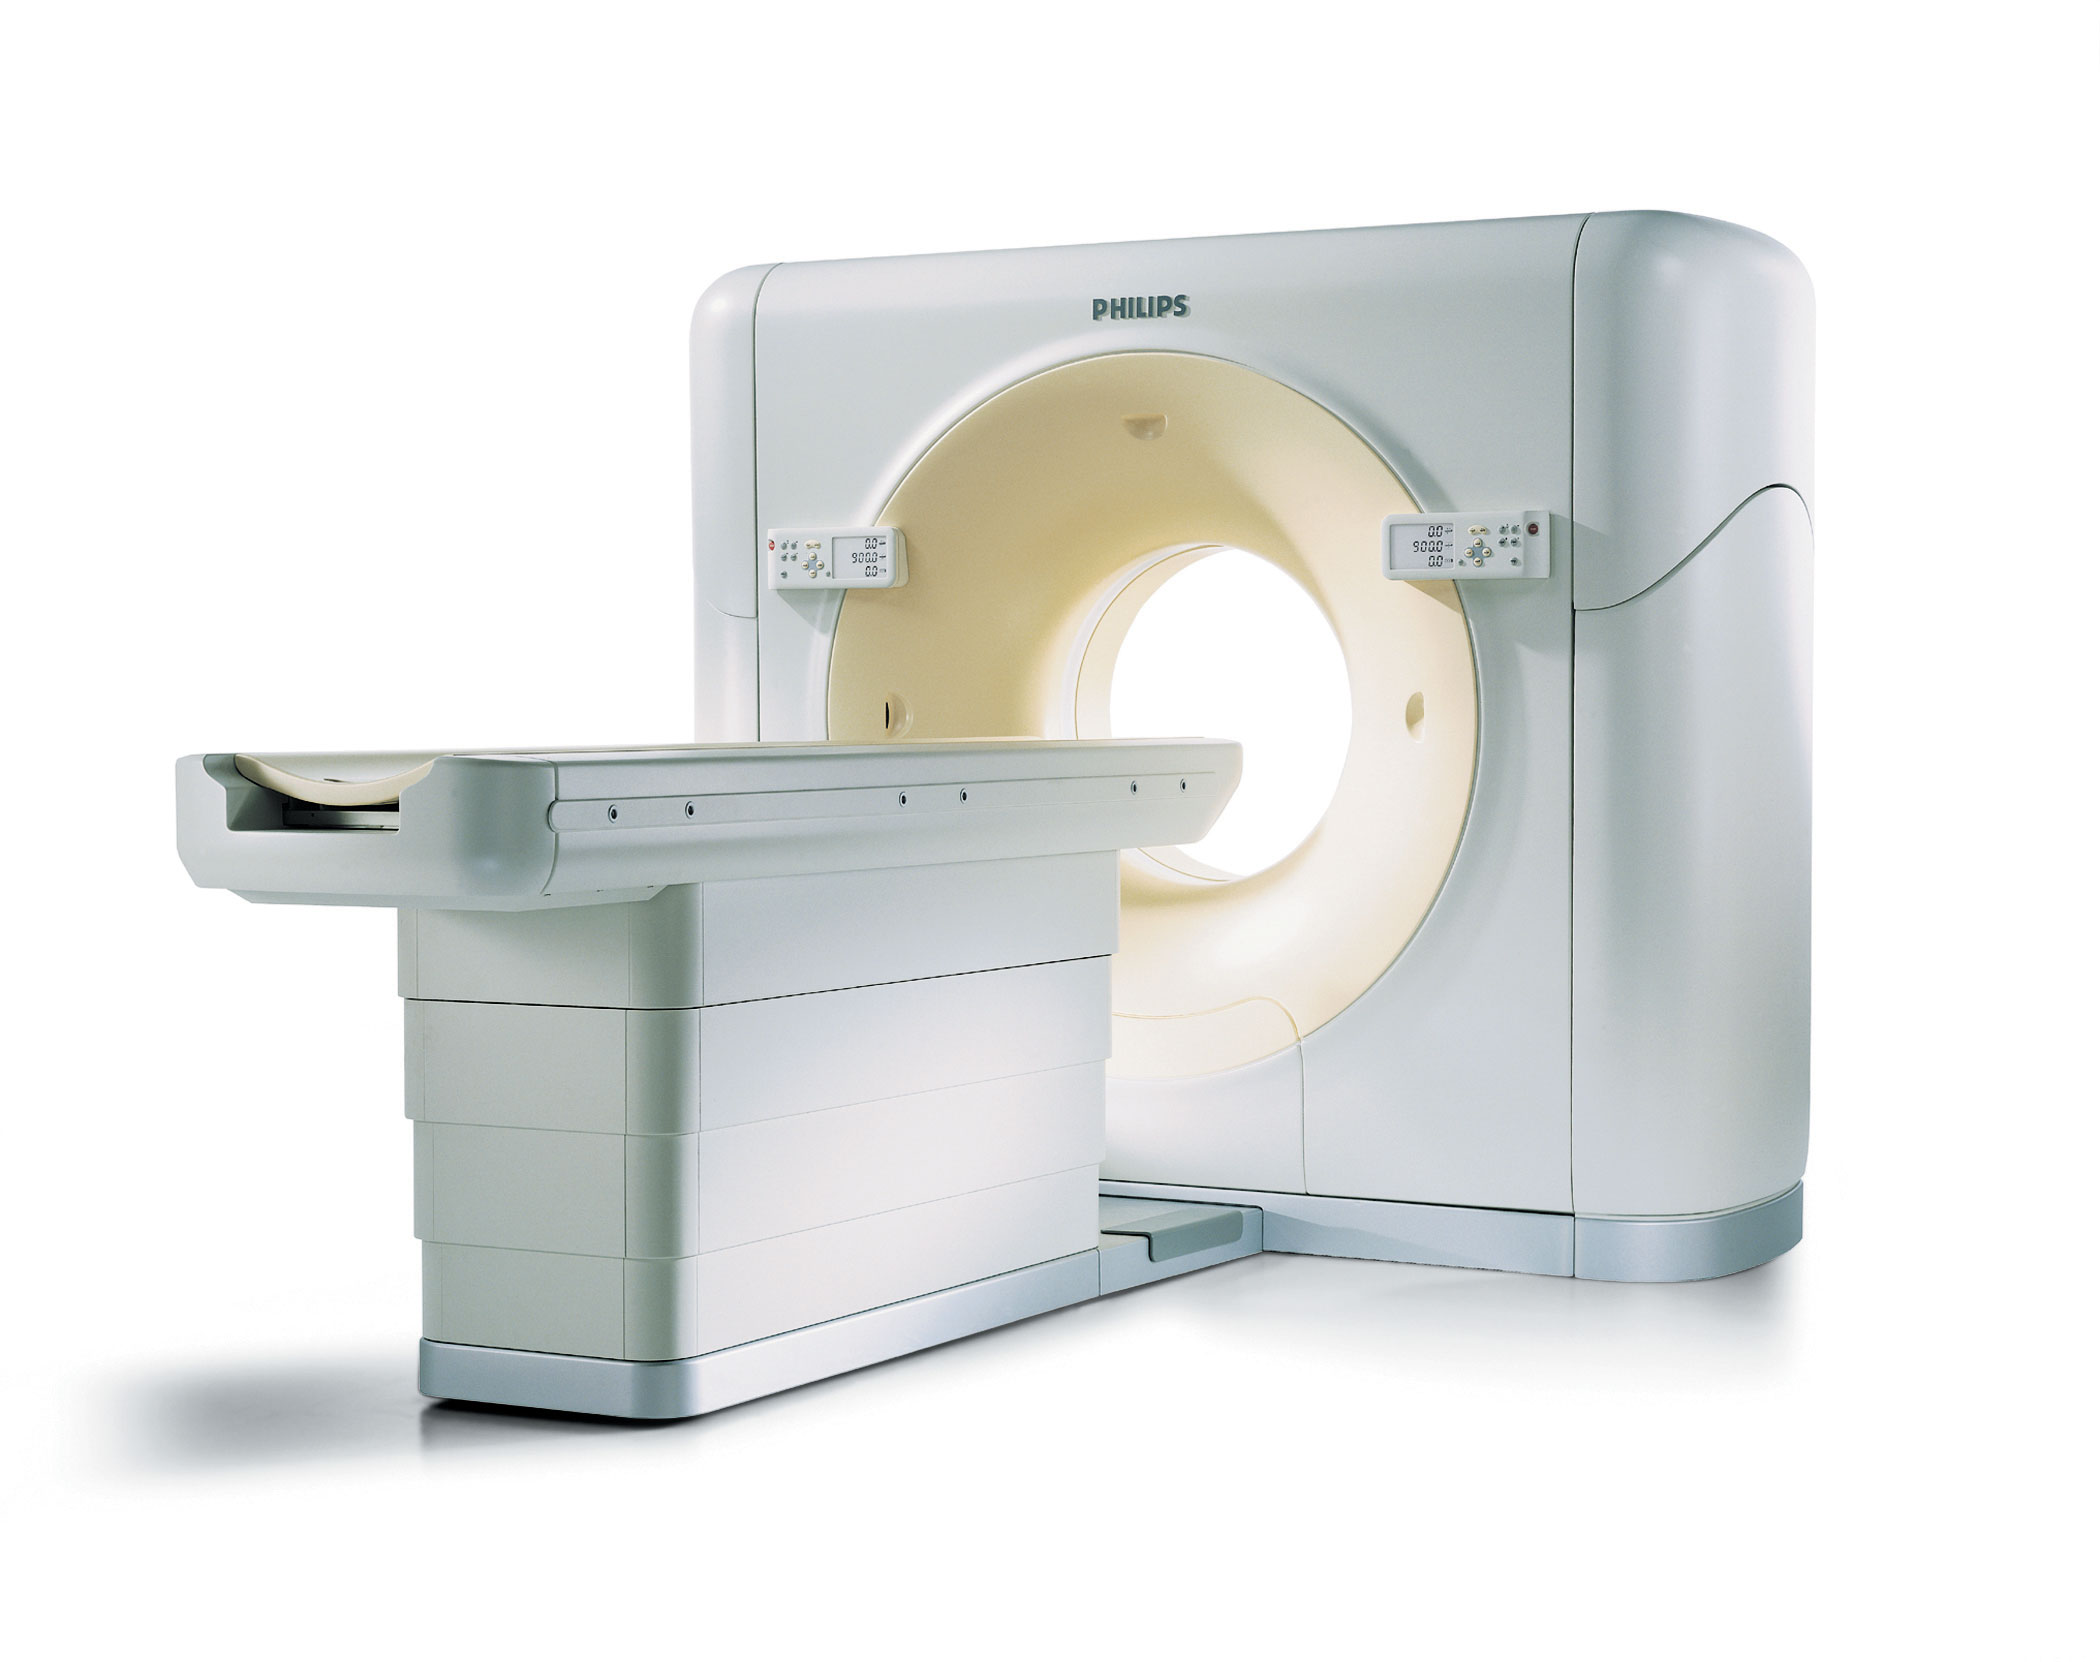
\includegraphics[width=\linewidth]{img/ctscanner.jpg}
  \caption{A CT scanner made by Philips. The patient takes place on the table
  and slowly slides through the toroid wherein the rotating X-ray
  source-detector pair is embedded.}
  \label{fig:ctscanner}
\end{center}
\end{figure}

\subsection{Technical background}
Just like radiographs, CT scanners are based on X-ray technology. They also
require a source and a detector, but this time they can rotate along the
patient. For every rotation angle $\theta$, we obtain an intensity profile
$I_\theta(r)$ along the axis $r$ perpendicular to the incoming X-rays (with
uniform intensity $I_0$). The family of functions $I_\theta$ can be transformed
into an attenuation profile $p(r, \theta) = -\ln \tfrac{I_\theta(r)}{I_0}$
(often called a sinogram). This $p(r, \theta)$ is called the Radon transform of
the attenuation distribution $\mu(x,y)$ in the slice plane.
\begin{equation}
	p(r, \theta) = \mathscr{R}\{ \mu(x,y) \}
\end{equation}

In short, the projections $p$ is what we can measure (or at least sample at
fixed intervals) and the attenuation distribution $\mu$ is what we are
interested in. The maths required to go from the latter to the former are pretty
straightforward, but the reverse is more complicated. The inverse Radon
transform $\mu = \mathscr{R}^{-1}(p)$ is needed.

We will not go into details, but the solution lies in the projection theorem.
This theorem states that the 2D Fourier transform $M(k_x, k_y)$ of $\mu(x,y)$
is equal to the 1D Fourier transform $P(k, \theta)$ of $p(r, \theta)$ (save for
a simple polar coordinate transformation).

\begin{equation}
\mathscr{F}_{1D}\{ p(r, \theta) \} = P(k, \theta) = M(k \cos \theta, k \sin
\theta) = \mathscr{F}_{2D}\{ \mu(x, u) \}
\end{equation}

Because the inverse Fourier transform is well understood, we have a solution to
our problem. Simple calculate $P$ from $p$ as explained above, and then apply
the inverse 2D Fourier transform to obtain $\mu$. By using the polar version of
the Fourier transform, we can reduce artifacts. This approach is called filtered
back projection \cite{suetens}.

After all the calculations are performed, we typically acquire a 512px $times$
512px scan. The values of the pixels in a CT scan are referred to as the CT
numbers and are expressed in Hounsfield Units (HU). They are calculated using
the fomula below, where $\mu$ is again the attenuation coefficient.
\begin{equation}
	\text{CT number} = \frac{\mu -
	\mu_{\text{H}_2\text{O}}}{\mu_{\text{H}_2\text{O}}} \cdot 1000
\end{equation}

From this, it becomes obvious that the CT number of air (with $\mu = 0$) is
-1000 HU and that the CT number of water is 0 HU. Bones on the other hand have a
very high attenuation coefficient and thus have a CT number in the thousands.
Soft tissue lies somewhere in between.

\subsection{Recent advancements}
The previous section assumed parallel X-ray beams. However, newer generation
scanners often employ cone-shaped beams. The procedure outlined above can
reconstruct a single slice by rotating around the subject by 180 degrees at a
time (a circular CT). On the other hand, modern CT scanners often spiral around
the patient while he moves through the toroid (a helical CT) to speed up the
process and thus decrease the exposure. Another useful trick is to capture
multiple slices at once by using multiple detector arrays. Until recently,
manufacturers were in a so-called \emph{slice wars} to offer the most detector
arrays. Needless to say, all this substantially complicates the mathematics
required to perform a back projection, but it is feasible and daily used in
hospitals around the world.

Another point of interest today is the combination of successive CT slices to
generate a 3D model of the patient. Because of advancements in computer
technology and algorithms, we can now post-process this 3D model to
automatically segment the bones and organs. This can for example help physicians
plan their actions before and during complex surgery.

\subsection{Future expectations}
Because CT scanners still require relatively high doses of radiation, this is
not an ideal solution. MRI scanners offer a safer alternative, but the large
magnetic fields produced make them impossible to use on patients with ferromagnetic
implants. Another advantage over MRI is the superior sub-millimeter resolution
that only CT scanners can handle. These are only some of the reasons why they
will not be replaced anytime soon. Future research will attempt to make CT scanners
even faster and allow them to produce clearer (i.e., higher contrast) images
with lower doses.

\section{Magnetic resonance imaging}\label{sec:mri}
While the previous imaging modalities were based on X-rays, Magnetic Resonance
Imaging (MRI) is based on magnetic fields. It is sometimes also referred to as
Nuclear Magnetic Resonance (NMR) in professional circles. However, the general
public has a certain aversion to the world ``nuclear'', so MRI is most used.
Instead of measuring the electromagnetic attenuation properties of various
tissue types as in CT scanners, we measure certain magnetic properties of the
tissue. These magnetic properties mainly depend on the molecular composition of
the material, for example on the amount of H$^+$ ions present (the proton
density). These electromagnetic waves are non-ionizing, meaning they cannot
cause cancer due to prolonged exposure. The goal is the same: imaging slices of
a patient's body. While technically an MRI scanner can generate slices in any
orientation without even moving the patient, CT-like cross sectional slices
are still used predominantly. Figure \ref{fig:mriscanner} shows a picture of an MRI
scanner.

\begin{figure}[ht]
\begin{center}
  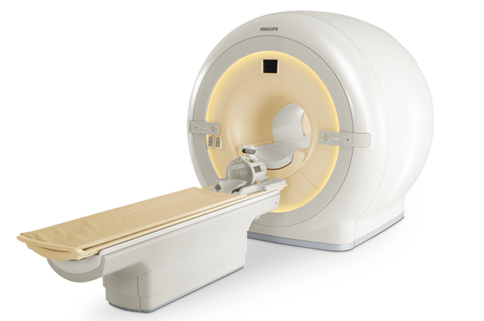
\includegraphics[width=\linewidth]{img/mriscanner.jpg}
  \caption{A Phlips MRI scanner. The patient takes place on the bed and is
  moved inside the toroid, but is not moved again during the procedure.}
  \label{fig:mriscanner}
\end{center}
\end{figure}

\subsection{History}\label{ssec:mrihist}
During the late 1960's, researcher in Aberdeen worked on the predecessor of the
modern MRI scanner \cite{mrihistory}. Their goal was to distinguish between
malignant tumors and normal tissue without using ionizing radiation. Instead of
measuring the magnetic properties of the nuclei, they initially focused on
electrons. This proved to be a dead end, and by early 1970 the group moved on to
NMR as we know it today. They realized that tumors have a longer $T_1$ time
(see below), and concentrated on that instead.

Meanwhile in the USA, chemist Paul Lauterbur proposed a way to create images
from NMR studies by using multiple field gradients to encode the position of
each measurement \cite{lauterbur1973}. Another important contribution came from
Peter Mansfield (now Sir), an English physicist. In 1974, he showed how to
select spins from a specific slice and patented a method to selectively excite
and define a slice across a sample. Lauterbur and Mansfield shared the 2003
Nobel Prize in Physiology or Medicine for their work on NMR.

From 1978 on, multiple research groups started presenting images generated by
prototype MRI scanners. However, only in the early 1980's was the technology 
ready for clinical and diagnostic use. By 1983, major multinational corporations
started producing commercial MRI machines.

\subsection{Technical background}
Unfortunately, the fundamental concepts that make MRI scanners work go beyond
classic physics, and instead requires special relativity, quantum mechanics and
quantum electrodynamics. Clearly, this is way beyond the scope of this text. We
will present a simplified version of the core principles based on
\cite{suetens} instead.

MRI scanners influence and measure the magnetic properties of atom nuclei in the
patient's tissue. During typical studies H$^+$ ions (i.e., protons) are used
because of their abundance in the human body, although alternatives exist
(e.g. ${}^{13}_6$C or ${}^{17}_8$O).

When the scanner is operational, a large magnetic field $\vec{B_0} = (0,0,B_0)$
(in the order of a couple Telsa) is induced along the patient's length using a
big electromagnetic coil. By supercooling the coil, the resistance drops and
power consumption can be reduced significantly.

The magnetic field $\vec{B_0}$ influences the magnetic moments $\vec{\mu_i}$ of
the nuclei, causing them to precess around the z-axis with precession frequency
$\omega_0 = f(B_0)$. Associated with the external magnetic field and the
individuel magnetic moments is the potential energy $E$. Quantum mechanics
states that for protons, this energy can only have two values, the so-called
spin up ($E_\uparrow$, lowest) and spin down ($E_\downarrow$, highest) state. In
these states, the $\vec{\mu_i}$ point respectively upwards ($u_z > 0$) and
downwards ($u_z < 0$), although transverse components are still present. Most
protons will be in the lowest energy state, but they can be flipped by absorbing
a photon with the appropriate amount of energy $\Delta E = E_\downarrow -
E_\uparrow$. This holds when the photon has a specific Larmor frequency
$\omega_{RF}$, which happens to be equal to $\omega_0$. In a 1T field, the
Larmor frequency for hydrogen is 42.6 MHz, a radio-frequency (RF) wave.

Of course, we are more interested in macroscopic voxels (3D pixels) than in the
individual nuclei. Fortunately, the net magnetization vector $\vec{M_0}$ of each
voxel is simply the sum of all individual magnetic moments $\mu_i$. The
magnitude of this vector roughly represents the proton density in the voxel. In
dynamic equilibrium, $\vec{M_0}$ points in the same direction as $\vec{B_0}$
because there are more nuclei in the spin up state and the individual transverse
components cancel each other out. To summarize: the large magnetic field made
sure the net magnetization vectors of all voxels are aligned. 

Unfortunately, due to technical reasons we can only measure the transverse
component of $\vec{M}$. As a solution, we will disturb the dynamic equilibrium
with a resonating RF pulse, causing more protons to flip to the spin down state.
This RF wave has a magnetic component $\vec{B_1} = (B_1, 0, 0)$. Following the
same logic as above, $\vec{B_1}$ causes $\vec{M}$ to precess around it. With the
appropriate timing, $\vec{M}$ can be flipped over an angle $\alpha$ of either 90
or 180 degrees.

After the pulse, the system returns to dynamic equilibrium during a process
called relaxation. We can distinguish between two effects. First, spin-spin
relaxation is responsible for the disappearance of the transverse component of
the net magnetization vector due to loss of phase coherence (increase in
entropy while energy stays constant). This process can easily be approximated
by a first order model with a time constant $T_2$, called the spin-spin
relaxation time.

\begin{equation}
M_{tr}(t) = M_0 \sin(\alpha) e^{-t/T_2}
\end{equation}

Different tissue types have different inherent $T_2$ times, which we will
exploit later.

\begin{figure}[ht]
\begin{center}
  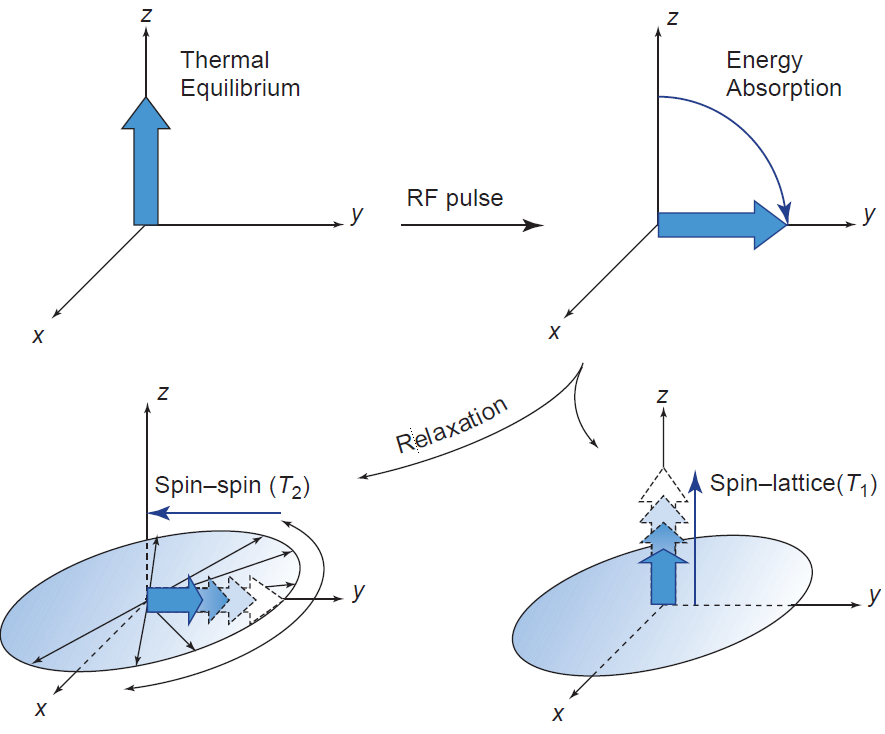
\includegraphics[width=\linewidth]{img/relaxation.png}
  \caption{Schematic overview of relaxation after a 90 degree pulse. \cite{suetens}}
  \label{fig:relaxation}
\end{center}
\end{figure}

Second, spin-lattice relaxation is responsible for regenerating the
longitudinal component of $\vec{M}$. Similarly, this process can be linked to a
$T_1$ relaxation time. $T_1$ is also a tissue property, and is always larger
than $T_2$.

\begin{equation}
M_l(t) = M_0 \cos(\alpha) e^{-t/T_1} + M_0 (1 - e^{-t/T_1})
\end{equation}

Using a quadrature detector in the xy-plane, we get the following reading
after one 90 degree pulse:
\begin{equation}
s(t) = M_{tr}(t) = M_0 e^{-t/T_2}
\end{equation}

To also measure $T_1$, we have to repeat the 90 degree pulse after repetition
time TR:
\begin{equation}
s(t) = M_0 (1 - e^{-TR/T_1}) e^{-t/T_2}
\end{equation}

Notice how the 90 degree pulse conveniently eliminates the sine and cosine
factors.

Clearly the result is not just the proton density $M_0$, but involves other
factors as well. This is not necessarily a problem as the $T_1$ and $T_2$
factors can increase the discriminative power of the scanner. If a short $TR$ is
chosen, the image is said to be $T_1$ weighted because long $TR$ times cause the
$T_1$ factor to diminish. If on the other hand a long $TE$ (echo time = moment
of measurement) is chosen, the image is said to be $T_2$ weighted. Indeed, a
short $TE$ time decreases the $T_2$ factor. By combining a long $TR$ with a
short $TE$, we have a relatively pure proton density image. Remember that $TR$
and $TE$ can be chosen by the operator, while $T_1$ and $T_2$ are tissue
dependent.

The attentive reader will have noticed that there is no spatial information
encoded in this signal yet. Using this approach we could only measure the
combined effects of all relaxations, which is useless. To solve this, we
superimpose additional gradients $\vec{G}_{x/y/z}$ (in the order of
milliTesla/meter) onto $\vec{B_0}$. This in turn affects the Larmor frequency.
The exact details are far from trivial and will be omitted, but involve the
3D k-space. After the signal has been sampled everywhere in the region of
interest in the k-space, a simple inverse Fourier transformation yields the
image we are looking for.

Using two 90 degree pulses is just one of the many possible pulse sequences used
in modern MRI scanners. Other examples include the spin-echo (SE) sequence and
the gradient echo (GE) sequence. Each sequence has advantages and disadvantages
with respect to discrimination of certain tissue types. The radiologist is
responsible for making the proper choice.

%fMRI (oxygen T2)
%flexible

\subsection{Recent advancements}
A lot of spin-off technologies based on MRI are in use. For example, Magnetic
Resonance Angiography (MRA) generates pictures of arteries to detect pathologies
such as stenosis (narrowing) or aneurysms (dilations). To make this work the
patient can be injected with a paramagnetic material. Alternatively, the scanner
can detect anomalies in the measurements due to movement of the blood, and
amplify those.

\hyphenation{me-ta-bo-lites}

Similarly, Magnetic Resonance Spectroscopy (MRS) measures the levels of various
metabolites in human tissue, while functional MRI (fMRI) visualizes brain
activity based on local oxygen levels. The underlying principle is that
oxygen-rich blood contains oxyhemoglobin, which is diamagnetic, while
oxygen-poor blood containing deoxyhemoglobin is paramagnetic. Likewise,
diffusion and perfusion can be measured.

\subsection{Future expectations}\label{ssec:mrifuture}
MRI scanners today are still far less ubiquitous than CT scanners, and only make
up a few percent of the worldwide radiographic examinations \cite{oecdhealth}.
However, because of the various advantages over other modalities - mostly the
fact that they use non-ionizing radiation - usage is expected to rise steadily
in the future. MRI will never completely replace CT because it cannot properly
image hydrogen-poor structures such as bone and air.

On top of that, future research will most likely improve the functional aspect
(e.g. measuring blood flow) of MRI. This can be done by experimenting with
nuclei other than hydrogen, by using new contrast agents and using novel pulse
sequences. In addition - similar to CT scanners - research will try to increase
the contrast and lower the acquisition times even further.

\section{Nuclear medicine imaging}
While the previous imaging modalities mostly focused on obtaining static images
of the patient, nuclear medicine imaging concentrates on so-called functional
imaging: visualizing some kind of process (e.g. drug metabolism) in the human
body. CT or MRI scanners also have this capability by exploiting certain side
effects of their underlying phenomena, but the Signal to Noise Ratio (SNR) is
always significantly lower.

Diagnostic nuclear medicine imaging works by tracking radioactive isotopes
(tracers)) as they move through the body. In the early days hospitals needed
their own cyclotron to produce these tracers, which significantly slowed
adoption. Nowadays various companies deliver the needed tracers daily to
hospitals around the world \cite{petreview}. Other variants of nuclear medicine
are used in the oncology departments to fight cancer, but we will not go deeper
into that.

Two main scanner types fall under nuclear medicine imaging: Positron Emission
Tomography (PET) and Single Photon Emission Computer Tomography (SPECT). The
exact difference will be explained later on in the technical background section.
\autoref{fig:petscanner} shows an example of a PET scanner.

\begin{figure}[ht]
\begin{center}
  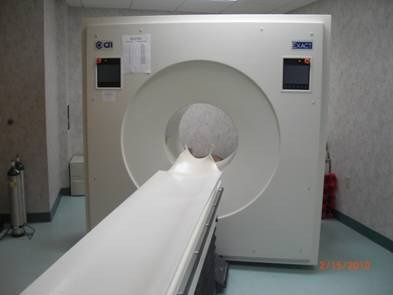
\includegraphics[width=\linewidth]{img/petscanner.jpg}
  \caption{A PET scanner made by Siemens. The opening is completely surrounded
  by detectors, so there are no moving parts inside.}
  \label{fig:petscanner}
\end{center}
\end{figure}

\subsection{History}
The history of nuclear medicine begins with the work of German physicist Hans
Geiger, a student of Ernest Rutherford, and his 1908 invention: the Geiger
counter. This device can detect ionizing radiation by exploiting the fact that
these rays can make an inert gas (e.g. Argon) conduct electricity. Using
this rudimentary device, researchers could form a rough picture of the radioactive
activity in a patient's body \cite{specthistory, geigercountertube}.

A significant breakthrough came with the invention of the Anger camera (or
gamma camera) in 1957 by Hal Anger, an American engineer and physicist. This
camera was able to detect incoming radiation from a whole organ at once,
improving the spatial resolution dramatically. The technique he used was based
on scintillator crystals \cite{anger}.

From there, several researchers such as Crandall, Cassen, Kuhl and Edwards built
upon the work to create true scanner systems throughout the late 1960's and
early 1970's. The first systems were SPECT scanners to make images in just one
plane, and later on CT-like scanners that could calculate cross sections were
invented.

Research concerning PET scanners was performed at about the same time
as SPECT scanners. Scientists soon realised their advantage, but adoption took
much longer in comparison \cite{petreview}. G. Brownell and his group were the
first to build a working dual planar PET scanner \cite{brownell}.

\subsection{Technical background}
Before we explain how PET and SPECT scanners work, we will quickly refresh some
important radioactive decay modes.

The first is positron emission, also called $\beta^+$ decay. Positrons (e$^+$)
are the anti-particles of electrons (e$^-$). During this decay, a proton (p$^+$)
inside an atom is essentially transformed into a neutron (n) and a positron.

\begin{equation}
	p^+ \rightarrow n + e^+
\end{equation}

\begin{equation}
	{}_Z^AX \rightarrow {}_{Z-1}^AY + e^+
\end{equation}

In the next couple of nanoseconds, the positron will fly into a electron and
annihilate. The mass of the two particles is is converted into pure energy in
the form of two photons ($\gamma$). Each photon carries 511 keV of energy and
they fly away in opposite directions.

This physical phenomenon forms the basis of Positron Emission Tomography (PET).
A typical element used during such studies is $^{18}$F, which has a half-life of
about 110 minutes. It yields stable $^{18}$O \cite{suetens}. The fact that two
photons are emitted is very convenient. If both happen to be detected, we
immediately know their projection line. (Remember that in CT scanners the
projection line is known a priori and is fixed between source and detector.)

The opposite operation is also possible: $\beta^-$ decay by electron emission.
Here, a neutron is converted into a proton and an electron.

\begin{equation}
	n \rightarrow p^+ + e^-
\end{equation}

\begin{equation}
	{}_Z^AX \rightarrow {}_{Z+1}^AY + e^-
\end{equation}

In certain cases, the resulting Y atom is in a metastable state ($^{Am}$Y).
This means the atom will later decay further into a more stable nuclear
configuration, releasing one or more photons in the process. This is much more
interesting diagnostic-wise, because unlike electrons, photons don't damage the
tissue they pass through during emission. A common metastable element
used is $^{99m}$Tc, generated after decay of $^{99}$Mo and with further decaying
into $^{99}$Tc (half-life of six hours) by decaying a single photon of 140 keV.

%electron capture

$\beta^-$ decay is mainly used in SPECT scanners. Because only one photon is
emitted, we cannot immediately tell where it came from when it is detected. To
solve this, a mechanical collimator - a thick lead plate with holes in it - is
used to absorb all photons that do not approximately fly perpendicular to it.
Knowing this, we can estimate the projection line of the photons we managed to
detect after they passed through the plate. Sadly, this technique forces us to
make a trade-off between spatial resolution (using smaller holes) and
sensitivity (letting more photons through using bigger holes). This is a serious
disadvantage compared to PET, in turn making SPECT less future-proof.

Note that these photons form electromagnetic waves, and their frequencies are
equal to or higher than those of the X-rays in earlier sections. This means that
they obey the same physical laws, and thus they also attenuate when passing
through tissue. However, in this context we refer to the radiation as
$\gamma$-rays instead.

When the photons are detected and the projection lines are calculated, we have
two options. Either we are satisfied with planar imaging to get a result similar
to basic radiography. In this case all depth information is lost, and the pixels
simply give information about the photon emission activity on their entire
projection line, combined with the attenuation properties of tissue on that
line. Sometimes a SPECT scanner is simply called a gamma camera in this
configuration, although the distinction is mostly theoretical. The other option
is to use a slightly adapted filtered back projection algorithm to compute
CT-like slices. Obviously this requires the detectors to rotate about the
patient just like in a CT scanner.

The detectors used here differ significantly from those used with X-rays. Not
only are there far fewer photons to be detected in the first place, but the
acquisition time is also much longer. Photomultiplier Tubes (PMT) combined with
NaI(Tl) scintillator crystals and, more recently, photo diodes are
popular detectors in use today.

\subsection{Recent advancements}
Due to the strong attenuation of the photons, filtered back projection produces
significant artifacts in the final image. The images are still diagnostically
relevant, but better methods are available. Iterative reconstruction based on
Bayesian statistics or maximum likelihood calculations are becoming more
popular.

Another advancement, the Time-of-Flight (TOF) PET scanner estimates the
source location of the photon along the projection line by measuring the
difference in arrival time of the two photons. This only works reliably if the
difference is smaller than 1ns, which in turn requires very advanced measuring
equipment.

While most researchers focus on nuclear medicine alone, others seek their
fortune in hybrid scanners. For example, combining CT or MRI with PET or SPECT
scanners significantly improves the specificity compared to their stand-alone
versions. Especially the PET/CT combination is popular in clinical environments.
In this case, the CT scanner can provide the attenuation correction needed for
the PET scanner. One problem that has to be overcome is the long acquisition
time needed for PET, and the mismatch it causes with CT scans due to patient
movement. Image registration techniques can be helpful here, but are not
straightforward.
\ldots

\subsection{Future expectations}
As with all types of scanners, we expect steady technological advancements in
the years and decades to come. However, in the case of nuclear medicine, experts
expect most progress to be made on the tracer front. This will enable researcher
to not only visualize biological processes on a macro level, but move to the
molecular level. This way, advanced studies on gene regulation,
radioimmunotherapy etc. will become possible.

%ultrasound, img processing, automated diagnosis

%ROC
